\level{2}{Processo di verifica}
		\level{3}{Verifica dei documenti}			
			\level{4}{Norme}
				\level{5}{Verifica dei documenti}
					Dare inizio all'attività di verifica di un documento è compito del \insrole{Responsabile di Progetto}: esso assegna il compito a uno o più \insrole{Verificatori}. Questi, con l'aiuto del diario delle modifiche, focalizzano la loro attenzione sulle sezioni del documento che sono state modificate.\\
Per eseguire una verifica quanto più accurata e completa possibile è necessario controllare che sia stato rispettato quanto segue:
					\begin{enumerate}
						\item sintassi semplice e corretta;
						\item periodi brevi e leggibili;
						\item struttura del documento;
						\item norme tipografiche;
						\item proprietà di glossario.
					\end{enumerate}
					Durante l'esecuzione dell'intera \insglo{procedura} di verifica dei documenti è importante che i \insrole{Verificatori} tengano traccia di tutti gli errori più comuni.\\ Questo può essere fatto seguendo la \insglo{procedura} descritta nella sezione \nameref{sec:tracciamento}.
					\level{6}{Sintassi}
						I \insrole{Verificatori} devono preoccuparsi di individuare gli errori sintattici all'interno dei testi del documento. Tale compito può essere in parte attuato tramite strumenti automatici, indicati nell'appendice \nameref{app:strumenti}. È tuttavia necessario che un documento sia sempre sottoposto a \textit{\insglo{walkthrough}}, in quanto gli strumenti automatici non sono in grado di individuare parole corrette che sono utilizzate al di fuori del loro contesto.\\ Inoltre, i \insrole{Verificatori} devono cercare tutte quelle parole che sono poco frequenti o comunque complesse (possono generare fraintendimenti o incomprensioni): va applicata la tecnica del \textit{\insglo{walkthrough}}.
					\level{6}{Periodi lunghi}
						I \insrole{Verificatori} devono calcolare l'\insglo{indice Gulpease} del documento (utilizzando l'apposito strumento automatico, vedi appendice \nameref{app:strumenti} del presente documento). Qualora si ottenga un risultato inferiore alle aspettative si deve applicare il \textit{\insglo{walkthrough}} all'interno del documento: l'obiettivo deve essere quello di individuare frasi troppo lunghe (e che dunque possono essere di difficile comprensione e/o scarsa leggibilità).
					\level{6}{Struttura del documento}
						I \insrole{Verificatori} controllano con l'ausilio di strumenti automatici (vedi sezione \nameref{app:strumenti} del presente documento) che la struttura del documento rispetti quanto descritto in questo documento.
					\level{6}{Norme tipografiche}
						Nel presente documento sono state definite delle norme tipografiche di carattere generale. Molte di esse sono verificabili tramite strumenti automatici (vedi sezione \nameref{app:strumenti} del presente documento). Per le restanti è necessario che i \insrole{Verificatori} applichino una fra le tecniche di \insglo{inspection} e \textit{\insglo{walkthrough}}	(si preferisce la prima nel momento in cui tramite la lista di controllo si riesce a trovare la grande maggioranza degli errori).
					\level{6}{Proprietà di glossario}
						È necessario che tutte le parole presenti all'interno del \insdoc{Glossario} siano marcate appropriatamente (come descritto nel presente documento). Ciò viene fatto con l'ausilio di strumenti automatici (vedi sezione \nameref{app:strumenti} del presente documento). Inoltre, è compito dei \insrole{Verificatori} trovare tutti quei termini che dovrebbero essere inclusi nel \insdoc{Glossario} ma che ancora non lo sono. Per tale compito si deve utilizzare \textit{walthrough} delle sezioni che sono state soggette a modifica prima dell'ultima verifica.

\level{4}{Procedure}
		\level{5}{Verifica dei diagrammi UML}
			I \insrole{Verificatori} hanno il compito di controllare tutti i diagrammi \insglo{UML} che sono stati prodotti. I diagrammi utilizzati fino a questo momento 
			sono i seguenti:
			\begin{itemize}
				\item diagrammi dei casi d'uso;
				\item diagrammi di attività.
			\end{itemize}
			\level{6}{Diagrammi dei casi d'uso}
				Le verifiche che devono essere effettuate riguardano sostanzialmente i casi d'uso e gli attori.\\
				Innanzitutto si deve controllare se un attore è davvero tale. Per fare questo può essere utile porsi domande descritte in seguito.
				\begin{enumerate}
					\item Il presunto attore in questione è una persona che interagisce con il sistema? Se la risposta è si allora esso probabilmente è un attore, se la risposta è no passare al punto due.
					\item Sono in grado di modificare il presunto attore all'interno del mio sistema? Se la risposta è no allora probabilmente è un attore, se la risposta è si allora probabilmente non si tratta di un attore.
				\end{enumerate}
				\begin{figure}[H]
					\centering
					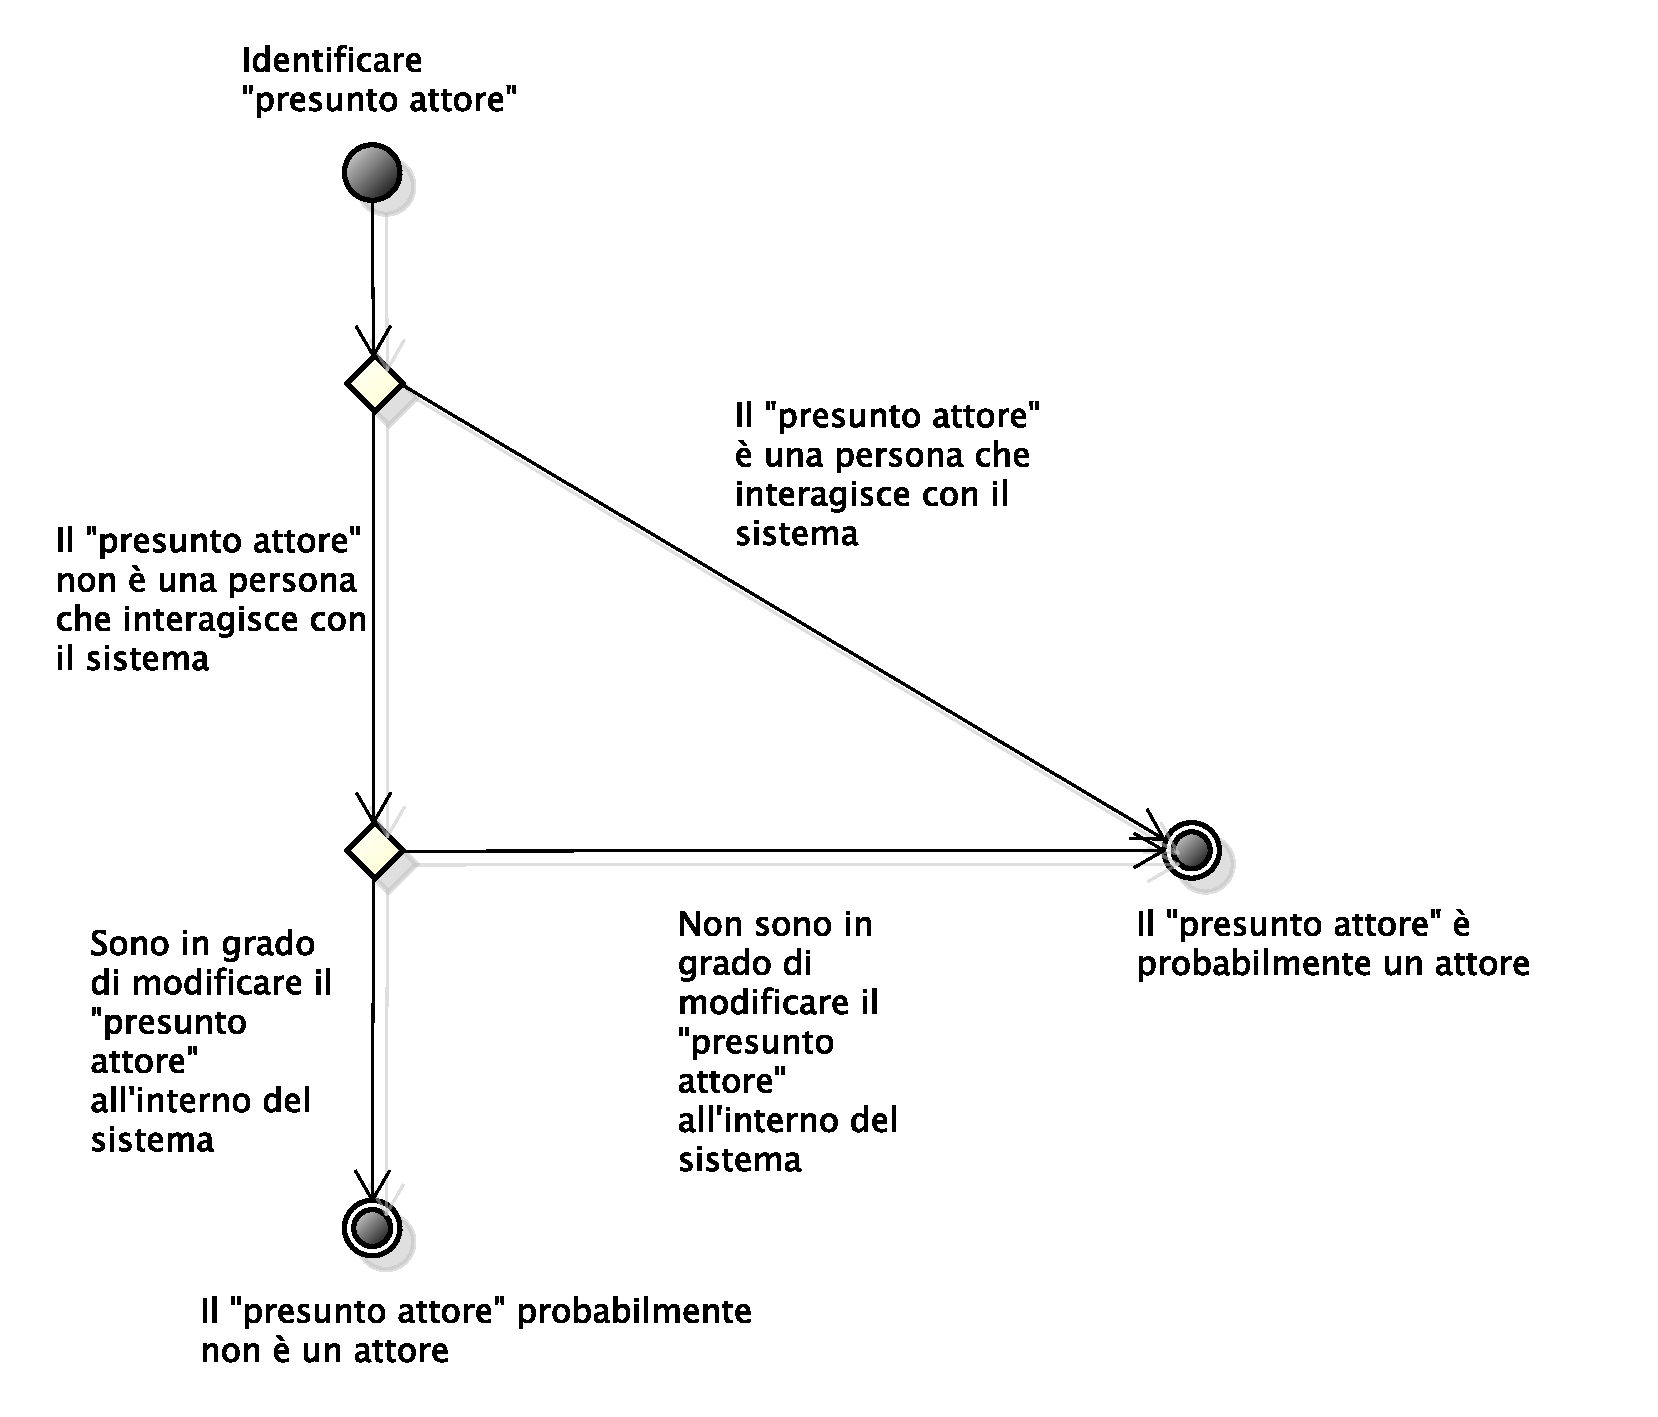
\includegraphics[width=0.6\textwidth]{NormeDiProgetto/Pics/VerificaAttori}
					\caption{Procedura per identificare un attore}
				\end{figure}
				Per quanto riguarda i casi d'uso, si controlla innanzitutto che siano utilizzate secondo lo standard \insglo{UML} le seguenti relazioni:
				\begin{itemize}
					\item inclusioni;
					\item generalizzazioni;
					\item estensioni
				\end{itemize}
				Infine, assicurarsi che i casi d'uso descrivano cosa il sistema fa e non cosa non fa.
			\level{6}{Diagrammi di attività}
				I diagrammi delle attività allo stato attuale delle cose sono stati usati esclusivamente per creare figure facilmente comprensibili che illustrino le procedure contenute nel presente documento. È dunque necessario verificare unicamente che tali diagrammi siano conformi allo standard \insglo{UML}.	
		
	
	\level{4}{Strumenti}
	Per l'attività di verifica dei documenti sono stati utilizzati degli appositi \insglo{script} sviluppati dagli amministratori e descritti nell'appendice \nameref{app:strumenti}.
\level{3}{Verifica del software}
\level{4}{Tecniche di analisi}
			Per poter determinare il livello di qualità del \insglo{prodotto} il \insglo{team} di sviluppo utilizza diversi tipi di tecniche di analisi dei dati.\\
			Queste possono essere suddivise in due grandi categorie:
			\begin{itemize}
				\item analisi statica;
				\item analisi dinamica.
			\end{itemize}
			\level{5}{Analisi statica}
				L'analisi statica è una forma di valutazione di un sistema o di un suo componente basato sulla sua forma, struttura, contenuto, documentazione senza che esso sia eseguito. Tali tecniche, dunque, sono applicabili tanto al codice quanto alla documentazione.
				Verranno usate le seguenti tecniche di analisi statica:
				\begin{description}
					\item[\insglo{walkthrough}] Tale tecnica viene utilizzata quando non si sa realmente cosa si sta cercando. Essa, infatti, consiste in una lettura da cima a fondo del documento/codice. Tale lettura ha lo scopo di trovare anomalie di qualsiasi tipo.
					\item[\insglo{inspection}] Tale tecnica viene utilizzata quando si ha un'idea di cosa si sta cercando e di cosa si potrebbe trovare. Essa consiste in una lettura mirata del documento/codice, sulla base di una lista degli errori comuni stilata in precedenza.
				\end{description}
				Applicare in modo fruttuoso la tecnica del \insglo{walkthrough} è molto oneroso e dispendioso. Tuttavia, quando non si possiede una lista degli	errori comuni (per esempio a inizio progetto), essa è l'unica soluzione. L'obiettivo è quello di formare una lista quanto più completa possibile di errori comuni in modo tale che possa essere eseguita quasi sempre la tecnica dell'\insglo{inspection}.
			\level{5}{Analisi dinamica}
				L'analisi dinamica è una forma di valutazione di un sistema \insglo{software} o di un suo componente basato sulla osservazione del suo comportamento in esecuzione. Tali tecniche, dunque, sono applicabili solo a componenti \insglo{software} e vengono svolte tramite l'esecuzione di test su essi.\\
				Deve essere preoccupazione di chi scrive i test fare in modo che essi siano di grande valore dimostrativo, in quanto il numero di test che devono essere effettuati è per forza di cose in numero finito e relativamente piccolo.
		\level{3}{Test}
					\level{4}{Test di integrazione}
					I test di integrazione servono per verificare il corretto funzionamento di più moduli assemblati insieme; in particolare servono per rilevare bug nei moduli nel momento in cui essi interagiscono con altri moduli coi quali hanno dipendenze.\\
					I test di integrazione vengono identificati dalla sintassi TI[Componente], dove Componente si riferisce al componente del sistema del quale si sta testando l'integrazione tra i suoi elementi.
					\level{4}{Test di sistema}
					I test di sistema validano i requisiti individuati nell'\insdoc{Analisi dei Requisiti v3.00}, ovvero validano il \insglo{prodotto} \insglo{software}, e vengono eseguiti dopo i test di integrazione.
					I test di sistema vengono identificati dalla sintassi TS[Codice del requisito], dove il codice del requisito è quello del requisito che sarà testato.\\
					Nel documento \insdoc{Piano di Qualità v6.00} vengono riportati i test di sistema relativi ai soli requisiti funzionali specifici.
					\level{4}{Test di accettazione}
					I test di accettazione avvengono al momento del collaudo del \insglo{software} col proponente.
					I test di accettazione sono identificati dalla sintassi TA[Codice del requisito], dove il Codice del requisito si riferisce al requisito che sarà testato.
		\level{3}{Issue tracking}
			L'\insglo{issue} tracking è un attività di supporto dei \insrole{Verificatori}. Essa permettere non solo di tracciare tutti i potenziali difetti dalla comparsa fino alla risoluzione, ma consente al \insrole{Responsabile di Progetto} di assegnare i compiti di correzione ai singoli membri del \insglo{team}.
			\level{4}{Norme}
				\level{5}{Sintassi delle label}\label{sec:SintassiLabel}
				Una label è una etichetta che viene applicata ad una \insglo{issue} utilizzando il servizio fornito da \insglo{GitHub} (consultare la sezione \nameref{app:strumenti} del presente documento) permettendo così di categorizzare e filtrare le varie issues.\\
				Esistono 3 tipologie di etichetta:
				\begin{itemize}
				    \item Di \textbf{attività}: ovvero quale attività l'ha generata. Le etichette permesse sono quindi: \inslabel{Verifica}
				    \item Di \textbf{appartenenza}: cioè da quale documento è stata sollevata la \insglo{issue}. Sono etichette valide tutte le etichette con nome la sigla dei documenti (seguendo la sintassi indicata nella sezione \nameref{sec:sigle}).
				    \item Di \textbf{stato}: identifica in che stato si trova la \insglo{issue}. Sono accettate solamente le seguenti etichette:
				\begin{itemize}
				    \item \inslabel{Request} identifica una richiesta di \insglo{issue};
				    \item \inslabel{Questioned} viene applicata ad una \insglo{issue} nella quale si sta discutendo al fine di trovare una soluzione;
				    \item \inslabel{ToDo} identifica che la \insglo{issue} è pronta per esser risolta con la soluzione accettata della discussione;
				    \item \inslabel{InProgress} rappresenta una \insglo{issue} alla quale il componente incaricato sta lavorando al fine di risolverla
				    \item \inslabel{Rejected} implica una \insglo{issue} respinta perché la richiesta è stata giudicata inutile o dannosa;
				    \item \inslabel{Done} identifica una \insglo{issue} completata.
				\end{itemize}
				\end{itemize}
			\level{4}{Procedure}
				\level{5}{Gestione di un'anomalia}
				Ogni qualvolta un \insrole{Verificatore} trova un anomalia deve segnalarla tramite il meccanismo di sollevamento \insglo{issue} fornito da \insglo{Github} (consultare la sezione \nameref{app:strumenti} del presente documento). L'intera \insglo{procedura} da attivare nel momento in cui viene individuata un'anomalia prevede i seguenti passi:
				\begin{enumerate}
				    \item il \insrole{Verificatore} crea una nuova \insglo{issue} su \insglo{Github} riguardante l'anomalia rinvenuta (seguendo la sintassi indicata nella sezione \nameref{sec:StrutturaIssue}) ed aggiunge come etichette \inslabel{Verifica}, quella relativa al documento/i interessato/i ed infine etichetta di stato \inslabel{Request} (si consulti la sezione \nameref{sec:SintassiLabel}).
				    \item il \insrole{Project Manager} valuterà la richiesta e se decide che la modifica è inutile o dannosa procederà cambiando etichetta da \inslabel{Request} a \inslabel{Rejected} e chiuderà la \insglo{issue} terminando così la \insglo{procedura}, in caso contrario cambierà l'etichetta da \inslabel{Request} a \inslabel{Questioned}, in modo che un qualsiasi componente del gruppo possa commentare, ribattere l'idea o proporne una nuova;
				    \item il \insrole{Verificatore} aggiorna la lista degli errori comuni (\insglo{procedura} descritta nella sezione \nameref{sec:tracciamento});
				    \item quando si è deciso che la soluzione proposta è quella ottimale (in caso entro 3 giorni dall'apertura della issue non si sia giunti ad una conclusione, il \insrole{Project Manager} sceglierà la soluzione migliore) l'etichetta verrà cambiata da \inslabel{Questioned} a \inslabel{ToDo} ed il \insrole{Project Manager} assegnerà il \insglo{ticket} di modifica ad un membro da lui scelto;
				    \item il componente scelto dal gruppo avrà il compito di modificare l'etichetta cambiandola da \inslabel{ToDo} ad \inslabel{InProgress} prendendo quindi in carico il \insglo{ticket} di lavoro;
				    \item effettuata la modifica, verrà inserito sul \insglo{repository} il risultato e verrà modificata la \insglo{issue} da \inslabel{InProgress} a \inslabel{Done} e verrà dunque verrà chiusa la \insglo{issue}.
			\end{enumerate}
			\begin{figure}[H]
					\centering
					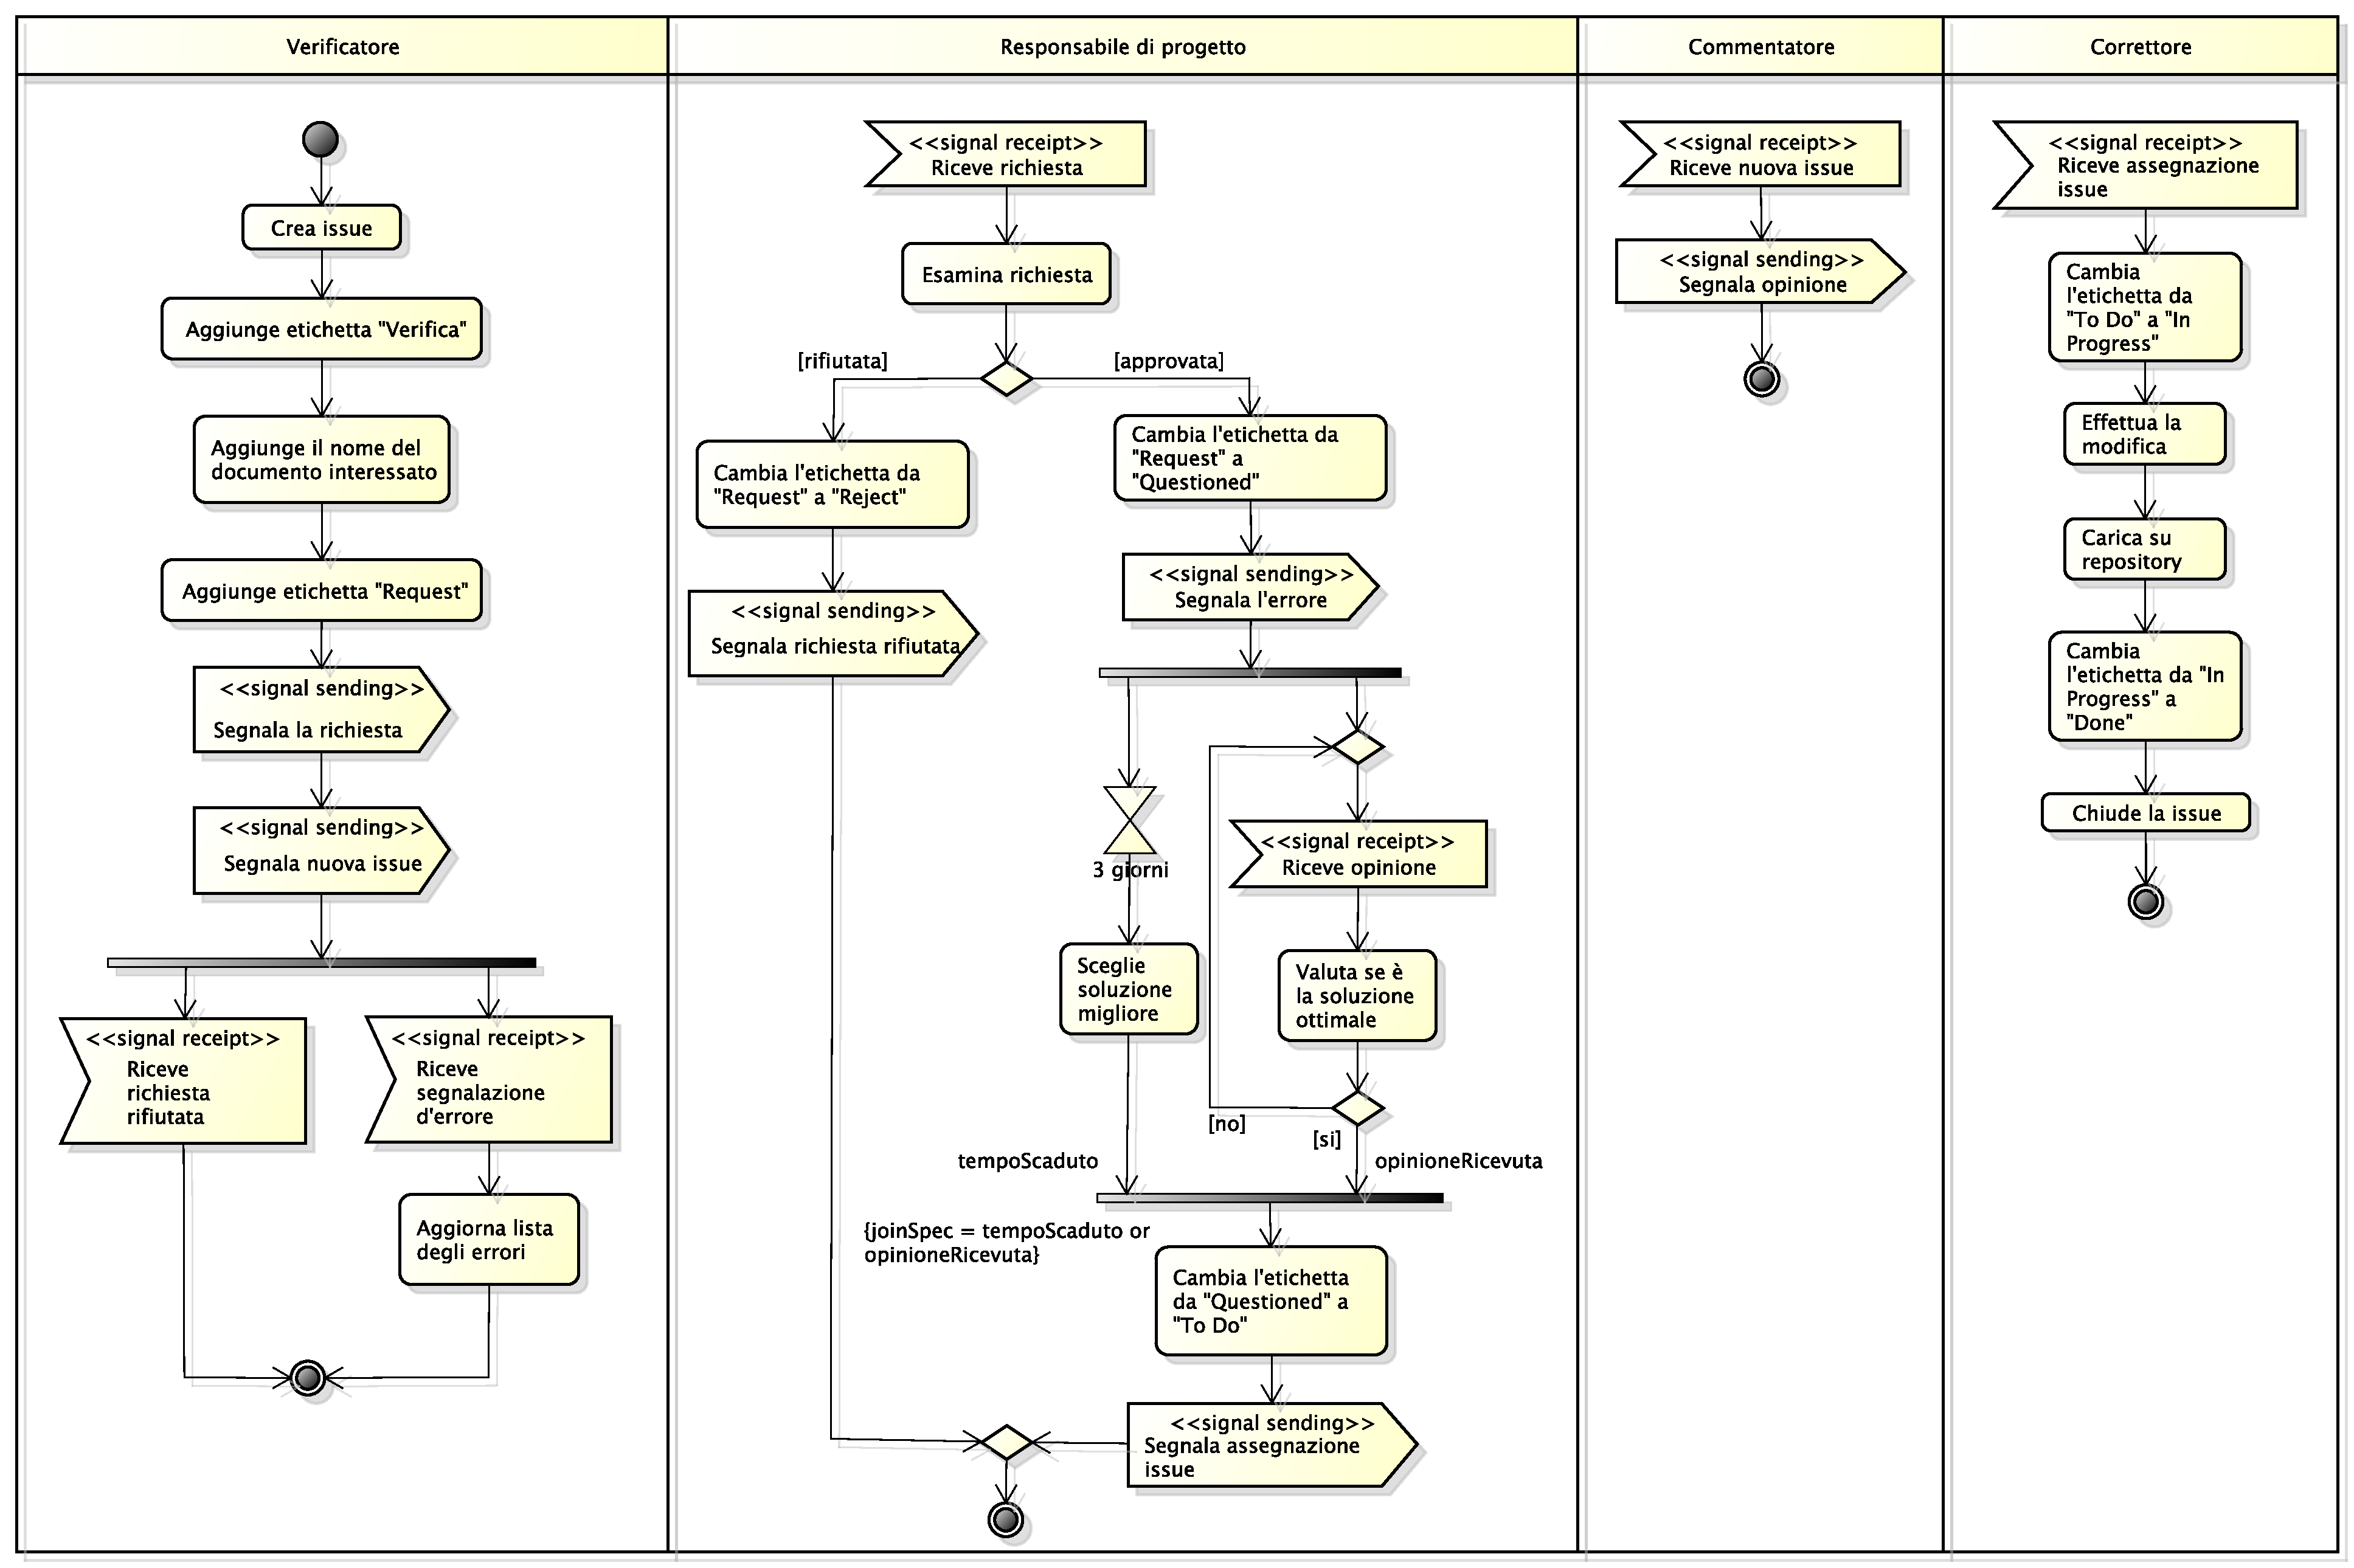
\includegraphics[width=1.0\textwidth]{NormeDiProgetto/Pics/GestioneAnomalia}
					\caption{Procedura di gestione di un'anomalia}
				\end{figure}
				\level{6}{Tracciamento degli errori più comuni nei documenti}\label{sec:tracciamento}
					È stata predisposta nell'applicativo Tracker una scheda con la possibilità di vedere e gestire la lista di controllo. Durante la \insglo{procedura} il \insrole{Verificatore} andrà ad incrementare il counter della voce relativa all'errore trovato, contribuendo a creare una statistica degli errori. Ci sarà quindi la possibilità per il \insrole{Responsabile di Progetto} di studiare l'andamento di questi ultimi e agire di conseguenza nel segnalare ai componenti del \insglo{team} eventuali situazioni particolarmente frequenti da evitare mentre si incrementano i documenti.\\ Il tracciamento costruito appositamente permetterà sia di applicare in modo fruttuoso la tecnica dell'\textit{\insglo{inspection}} grazie alla lista di controllo, sia di migliorare la prevenzione sistematica degli errori più critici in \insglo{fase} di creazione dei documenti di progetto.
					\begin{figure}[H]
							\centering
							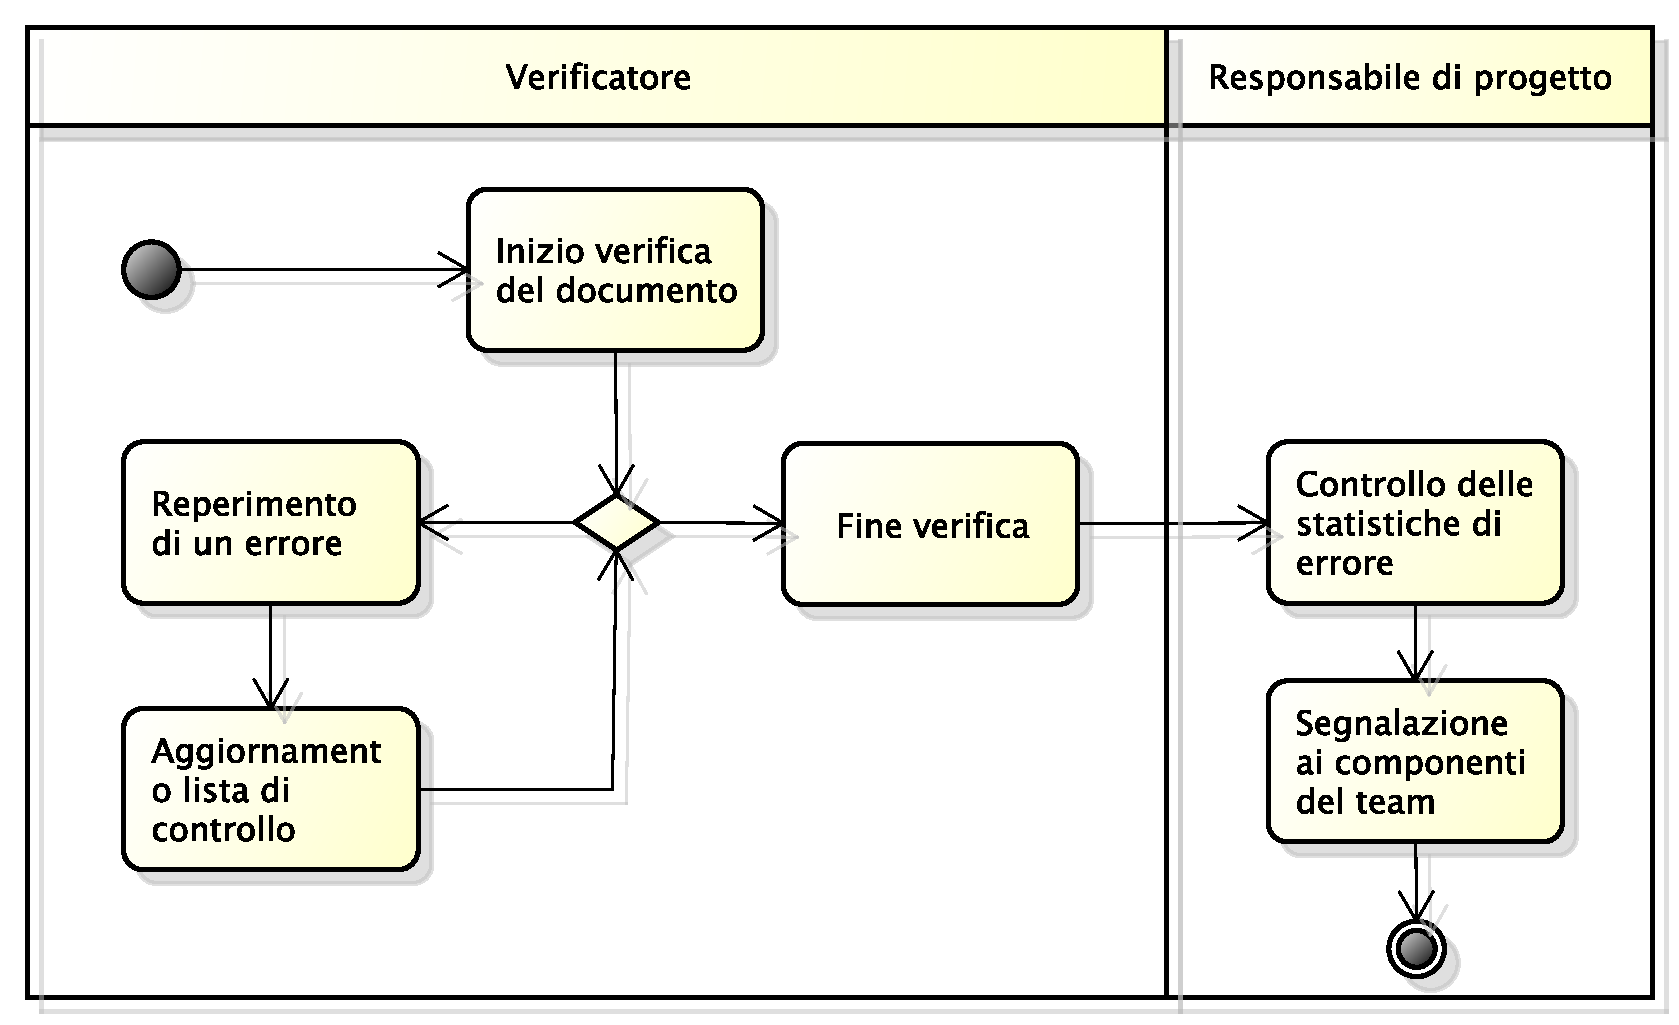
\includegraphics[width=0.6\textwidth]{NormeDiProgetto/Pics/ProceduraDecrementoErrori}
							\caption{Procedura per tracciamento errori comuni}
					\end{figure}
		\level{4}{Strumenti}
			Per la gestione delle \insglo{issue} è stato deciso di appoggiarsi al servizio di \insglo{issue} tracking offerto da \insglo{GitHub}, come suggerito nel \insglo{capitolato}, in modo da unificare gestione delle \insglo{issue} e versionamento. \\
			Viene poi utilizzato un servizio fornito da \textit{Tracker}, ovvero un'applicazione web creata dal \groupname, per permettere al \insrole{Project Manager} di avere una visione statistica degli errori effettuati dal \insglo{team}.
